%!TEX root = ../tommaso-thesis.tex
%!TEX spellcheck = en_US


% \chapter{Blended, Not Stirred: \\Multi-concern Visualization of \\Large Software Systems}\label{ch:blend}
\coolchapter{Blended, Not Stirred}{Multi-concern Visualization of Large Software Systems}{ch:blend}


While constructing and evolving software systems, developers generate directly and indirectly a large amount of data of diverse nature, such as source code changes, bug tracking information, IDE interactions, stack traces, etc.
Often these diverse data sources are processed and visualized in isolation, leading to a partial view of systems.

We present a \emph{blended} approach to visualize several data ``ingredients'' at once, to give as complete an answer as possible to the question {``What happened to the system in the last few days?''}.
The goal is to enable a quick and comprehensive assessment of what happened to a software system in any given time frame.

\structure

% \secref{sec:blend-related} presents the related work.
In \secref{sec:blend-ingredients} we describe the ingredients of our blended visualization, which is presented in \secref{sec:blend-visualization}.
In \secref{sec:blend-stories} we use the visualization to tell interesting evolutionary stories.
Finally, \secref{sec:blend-summary} summarizes and concludes the chapters.

\newpage


%%%%%%%%%%%%%%%%%%%%%%
\section{Exploring a System} \label{sec:blend-intro}
%%%%%%%%%%%%%%%%%%%%%%

Software development involves a variety of activities carried out with a number of tools, components and environments, that relate to many different aspects of a system.
The increasing size of software projects, the increasing popularity of distributed development platforms like \texttt{GitHub}\seeurl{https://github.com}, and the amount of tools and frameworks available for every language, turned a significant part of modern software development into an integration process, where the developer can define a behavior by orchestrating and specializing library components and third-party entities.
This has turned the engineering of any software system into an information-heavy process, which is ultimately distilled into (hopefully functional) source code.
The vast majority of the corollary information (such as discussions, design decisions, email communication between developers, bug reports, etc.) is either discarded or ignored.
This is in part due to its often only semi-structured nature, where structured fragments are interleaved with natural language.
The mining of such unstructured data has become a research field of its own in the past few years.

When it comes to the understanding of any system, the natural focus is the source code, and indeed it --and the overarching structure and architecture-- has been the primary subject of study of program comprehension research.
In the context of software visualization many approaches have been developed to visualize the (evolving) structure of software systems, which range from static visualizations to historical or dynamic ones.
What strikes in this context is that many approaches consider only single concerns, such as the architecture, the structure, the evolution, the relationships, etc., but there is little in terms of visualizing multiple concerns at once.

We present here an approach to visualize multiple concerns concurrently.
The concerns we tackle are interaction data, failure information, and evolution.
Interaction data stems from how developers interact with the integrated development environment (IDE) while developing and maintaining a system.
In essence, it provides evidence of where and how people have been active while developing~\cite{Mine2015b}.
Failure information is generated each time the debugger is triggered because an exception has been raised.
In our previous work we have shown that such data can be leveraged to understand where the particularly tricky spots in a software system are located~\cite{DalS2015a}.
Both interaction data and failure data are more fine-grained than their respective counterparts, namely versioning information and bug reports.
We complement these two types of data with a third one, the evolution of the system.

Although we focus on these types of information, our approach can be extended to feature any kind of information artifact related to a large software system under development.
In essence, our goal is to answer one of the most often asked questions raised by developers and managers alike, namely ``what happened to our system recently''?~\cite{Sill2008}

We present a visual approach to \emph{blend} development data originated by different  sources, \eg by different tools that record and persist code changes, interaction data and stack traces.
We propose an interactive map that summarizes the relevant events that involved the system in a given period of time, using the city metaphor to represent a software system~\cite{Wett2007}, and coloring each entity according to the combination of data gathered around it.
We allow to explore the evolution of the system by navigating the information during time, and refining the search of interesting events to specific moments.
We then present some stories obtained through our visualization that illustrate interesting properties of an existing software project and its community.

The contributions we present in this chapter are:

\begin{itemize}

\item A novel approach to visualize multiple concerns concurrently in large scale software systems.

\item The supporting tool infrastructure to mine and integrate the data stemming from various sources of information.

\item Initial anecdotal evidence that our approach indeed allows us to discover and investigate facts that would otherwise remain hidden in the literal ``sea of data'' that surrounds any large and long-lived software system.

\end{itemize}


% \section{Related Work}\label{sec:blend-related}
%
% Many researchers showed how using data generated during the programming activity can provide valuable information about the evolution of a project.
%
% For example, Bacchelli et al.
% proposed an Eclipse plugin to integrate email communication in the IDE~\cite{Bacc2011a}.
% They showed that having the email data produced during the development of a software system at one's disposal helps supporting program comprehension tasks, such as finding entry points in a system and recovering additional documentation.
% %For example, Bacchelli \etal proposed a popularity metric based on the volume of discussion generated by software entities in development mailing lists, and showed that this information, correlated with source code and change metrics, helps in improving the predictive powers of defect prediction techniques~\cite{Bacc2011a}.
% Another example has been given by Zimmermann \etal, who applied data mining techniques to version histories to detect changes and build prediction model to suggest future changes to developers~\cite{Zimm2004a}.
%
% To effectively present and understand such an amount of data, many researchers and practitioners are adopting visualization and \emph{Visual Storytelling} approaches.
% The ability of contextualizing the information in a story that explains the meaning of the data is becoming more and more central to the skills required to data scientists~\cite{Segel2010a}.
%
% Among the different visualizations that researchers used to represent a software system, the city metaphor has proven to be effective in giving a high level picture of a group of entities, allowing the user to navigate, zoom and inspect the various components and refine the view~\cite{Wett2011a}.
% This approach has been adopted in different scenarios, depicting different kind of information pertaining several steps of the development activity, such as changes in the system, the defects involving different components in the system, issues in quality checking rules or the exceptions in the system~\cite{Panas2003a}.
%
% Other visualization approaches tried to focus on the evolution of software systems, specifically the version repositories, the dependencies or the structures.
% For example, Fischer \etal~\cite{Fisch2006a} proposed EvoGraph, an approach based on data extracted from a system release history, that visualizes the evolution of structural dependencies through 2D visual representations.
% Girba \etal~\cite{Girb2005a} focused on the visualization of the evolution of class hierarchies, correlating the history of classes and their relationships, \eg inheritance.
% The approach by Voinea \etal~\cite{Voin2007a} uses a combination of color and texture to represent as many attributes as possible to display information extracted from software configuration management systems.
% Another important approach is the one by Ratzinger \etal~\cite{Ratz2005a}, that represents systems as nested, zoomable graphs.
%
% However, while these approaches effectively visualize data about a single aspect that impacts or involves a system, they fall short in correlating this information with knowledge coming from diverse data sources and impacting diverse concerns.
% Such additional information could effectively integrate the existing data to uncover further relations between the elements of the system.
%
% We think that an approach that considers more than one kind of data and presents the information in a unified, uniform view, normalizing and balancing each source, could provide a greater value in understanding a software project and the activities happening in its ecosystem.



\section{The Ingredients}\label{sec:blend-ingredients}

%As per the title of our paper, \emph{``Blended, Not Stirred''} our visualization presents a blend of different ingredients to enable analysis from different, maybe orthogonal, perspectives.
In this section we briefly describe the three main ingredients together with the tools that enable the data collection process.

%As per the title of our paper, \emph{``Blended, Not Stirred''}, our visualization presents a composition of different information, obtained by blending together different data sources to enable analysis from etherogeneous and multidimensional perspectives.
To get a tractable subset of meaningful data, we decided to focus on a timespan ranging from January 1st 2015 to May 1th 2015.
In this section we present the context of our analysis, then we briefly describe the three main ingredients together with the tools that enable the data collection process.
Our visualization presents a composition of different information, obtained by blending together different data sources and enabling visual analytics from heterogeneous and multidimensional perspectives.
To get a tractable subset of data, we focus on a timespan ranging from January 1st 2015 to May 1th 2015.
In the rest of the section we describe the three main ingredients together with the tools that enable the data collection process.
For further details about the \pha platform see \appref{ch:pharo}.

% \subsection{The Pharo Ecosystem} \label{sec:blend-ingredients:pharo}
%
% \pha is a Smalltalk inspired programming environment, composed of the \pha programming language, an integrated development editor and a set of libraries covering the common needs for the daily programming tasks.
%
% Apart from a rich software collection, the \pha ecosystem is composed of a vibrant and active community\seeurl{http://pharo.org/community} that includes about 2,000 developers both from academia and industry.
% The community actively participates in the development of the system by building tools to improve the user experience, submitting bug reports and proposing patches to solve defects.



\subsection{Source Code Changes}\label{sub:changes}

A typical metric that is often considered in evaluating the growth and evolution of a system is the number of changes that it goes through during its development.
In the case of \pha, the whole system is self-contained and distributed as an \emph{image}, a single file that works as a virtual environment where new code is installed inside the default system.
The \pha system is released once a year, and during this period it goes through an intense phase of improvement, debugging and polishing.
The test and release process is managed by a continuous integration server,\seeurl{https://ci.inria.fr/pharo/} that stores the previous builds of the system.
In our analyses we modeled and extracted all the source code changes between subsequent releases of the \pha system.


\subsubsection{Retrieving the different version}

We focused on the release of \pha 4, which just finished its release cycle.
We downloaded all the development versions from the file server,\seeurl{http://files.pharo.org/image/40} that we also used to retrieve the exact release date of each version.
The full cycle of development images ranges from version $40,000$ to the image $40,613$, from May 26th 2014 to May, 5th 2015.
The last release in date May 1th 2015 was version $40,611$.


\subsubsection{Extracting a system model}

We extracted from each image a model representation of the system.
Such a model is composed of the names of all packages, classes, instance and class methods, and instance and class attributes.


\subsubsection{Generating an incremental change model}

We leveraged each system model to obtain an incremental diff model that describes each change.
We considered as change a variation in the names of the collected entities.
Since we had no way to precisely determine when an entity was renamed, we considered every event in terms of creation and deletion.
\tabref{tab:pharo} summarizes the available source code changes data.

%Source code changes represent the last ingredient of our \emph{``visual cocktail''}.
\pha, the target IDE of our study, is an open-source system maintained by an active community.
During its evolution it undergoes a series of minor and major releases, managed by a continuous integration server\seeurl{https://ci.inria.fr/pharo/}.
In our analyses we modeled and extracted all the source code changes between subsequent releases of the system.
\tabref{tab:pharo} summarizes the available source code changes data.

\begin{table}[ht]
  \center
  \caption{Source Code Changes}
  \label{tab:pharo}
  % \rowcolors{2}{gray!12}{white}
  %\def\arraystretch{1.1}
  \begin{tabular}{lr}

  % \rowcolor{gray!30} \textbf{Version} & \textbf{Added} & \textbf{Modified} & \textbf{Deleted} & \textbf{Tot.} \\ \hline
  % number of versions considered & 551 \\

  % \rowcolor{gray!30} \textbf{Metric} & \textbf{Value} \\ \hline
  % Number of considered versions & 611 \\
  % Number of changes & 4,928 \\
  % Average changes per version & 8 \\
  % Max number of changes per version & 527 \\
  % Min number of changes per version & 0 \\
  \textbf{Metric} & \textbf{Value} \\ \hline
  Number of considered versions & 611 \\
  Number of changes & 4,928 \\
  Average changes per version & 8 \\
  Max number of changes per version & 527 \\
  Min number of changes per version & 0 \\

  %4.0a & 10 & 10 & 10 & 30 \\
  %4.0b & 10 & 10 & 10 & 30 \\
  %4.0c & 10 & 10 & 10 & 30 \\
  %4.0d & 10 & 10 & 10 & 30 \\
  \end{tabular}
\end{table}



\subsection{\slr and Stack Traces}\label{sub:stacktraces}

A consistent part of the time spent by developers consists in finding and solving defects.
The debugging activity involves tests to reproduce a problem or verify that a defect has been solved.
This process generates many stack traces, that contain valuable information about the failures in a system.
Such information is normally used by a developer to identify a faulty status in her program.
Moreover, if collected and stacked together, stack traces can also give a hint of what parts of the system are the most active, or which ones are causing more troubles.
To exploit this source of information, we developed \slr~\cite{DalS2015a}, a platform to collect and store stack traces generated by the whole \pha community.
The data we collect contains the signature of every method invocation, to keep track of each entity involved in the failure, though excluding the method parameters, to avoid privacy issues for the single developer.

In enabling the reporter, each developer can decide to inspect each stack trace and choose the ones to submit, or enable the automatic reporting feature and submit all the traces produced by its activity.
While this option produces many duplicates and non relevant data, it is still interesting to see where the activity of the developers focuses in different periods of time.
The collected data can then be used to aid the debugging activity, for example detecting if a large volume of new stack traces coming from different developers involve a specific class, or by looking for existing bug reports in the bug tracker to provide a contextual help when a user encounters an exception and ease the understanding of a piece of code.
The presence of many different stack traces for a specific component might also suggest that an API has a problematic design, and that the users struggle in understanding its usage, thus highlighting the need for documentation or refactoring.

\tabref{tab:stacktraces} summarizes the collected and available data for stack traces.

\begin{table}[ht]
\caption{Stack Traces Data}
\label{tab:stacktraces}
\rowcolors{2}{gray!12}{white}
%\def\arraystretch{1.1}
\begin{tabularx}{\linewidth}{X|r}

\rowcolor{gray!30} \textbf{Metric} & \textbf{Value} \\ \hline Number of traces & 14884 \\
 Number of submitters & 43 \\
 Total number of stack trace lines & 714,420 \\
 Average stack trace size (in lines) & 48 \\
 Longest stack trace & 1,086 \\
 Shortest stack trace & 1 \\
\end{tabularx}
\end{table}




\subsection{\dfl and IDE Interaction Data}\label{sub:interaction}

During the process of software construction and evolution, supported by integrated development environments (IDEs), developers generate a large amount of data known as \emph{``IDE Interaction data''}~\cite{Kers2005, Murp2006}.
Examples of such data include \begin{inparaenum}[i)] \item \emph{IDE meta events}, like adding a method to a class, saving some edited code, or inspecting a variable in the debugger, \item \emph{UI events}, like moving a window or a tab in the IDE, or resizing them, and \emph{low-level events}, like keystrokes, mouse clicks, drags and simple movements\end{inparaenum}.

Since current IDEs do not record these data, in our previous work we developed \dfl, a silent interaction profiler for the \pha IDE~\cite{Mine2015b}.
\dfl records 32 different types of events at different levels of abstraction.
For this work we only focused on a subset of meta events that involve code entities.
Some meta events have an associated program entity: A browse event, for example, where the user opens a new code browser, can be performed on a method or on a class.

For this work we aggregated all meta events to the class-level: An event performed on method \texttt{foo} of class \texttt{Bar} counts as an event involving directly the class \texttt{Bar}.
In total we have ca.
239,000 interaction data events covering a timespan of 4 months (\ie from January to April 2015).

The IDE interactions impact 2,988 different classes, of which 965 are part of the standard \pha distribution.
The remaining 2,023 classes are user defined classes that are outside the scope of our study.
Out of the 32 types of meta events recorded with \dfl~\cite{Mine2015b}, only 13 types of events appear in the dataset.
This is because some of the recorded meta events do not carry any information related to program entities.
For example, the meta event that represents the opening of a \texttt{Finder}, a user interface used in \pha to search for pieces of code, has no associated program entity.

\tabref{tab:idata} summarizes the dataset and provides additional details.

\begin{table}[ht]
\caption{IDE Interaction Data}
\label{tab:idata}
\rowcolors{2}{gray!12}{white}
%\def\arraystretch{1.1}
\begin{tabularx}{\linewidth}{X|r}

\rowcolor{gray!30} \textbf{Metric} & \textbf{Value} \\ \hline
Number of Interaction Events & 238,741 \\
Number of Developers & 18 \\
Number of Interested Classes (in the \pha distro) & 2,988 (965) \\
Number of Different Event Types (total) & 13 (32)
\end{tabularx}
\end{table}



\subsection{Blended, Not Stirred}

Our goal is to develop a visualization approach which can represent diverse data sources, such as the ones we just presented.
The approach is not geared towards the specific types of sources, and also not limited to depicting just those, but is in principle extensible to feature any number and any source of data.



\section{Visualization Principles}\label{sec:blend-visualization}

\begin{figure*}[ht]
\centering
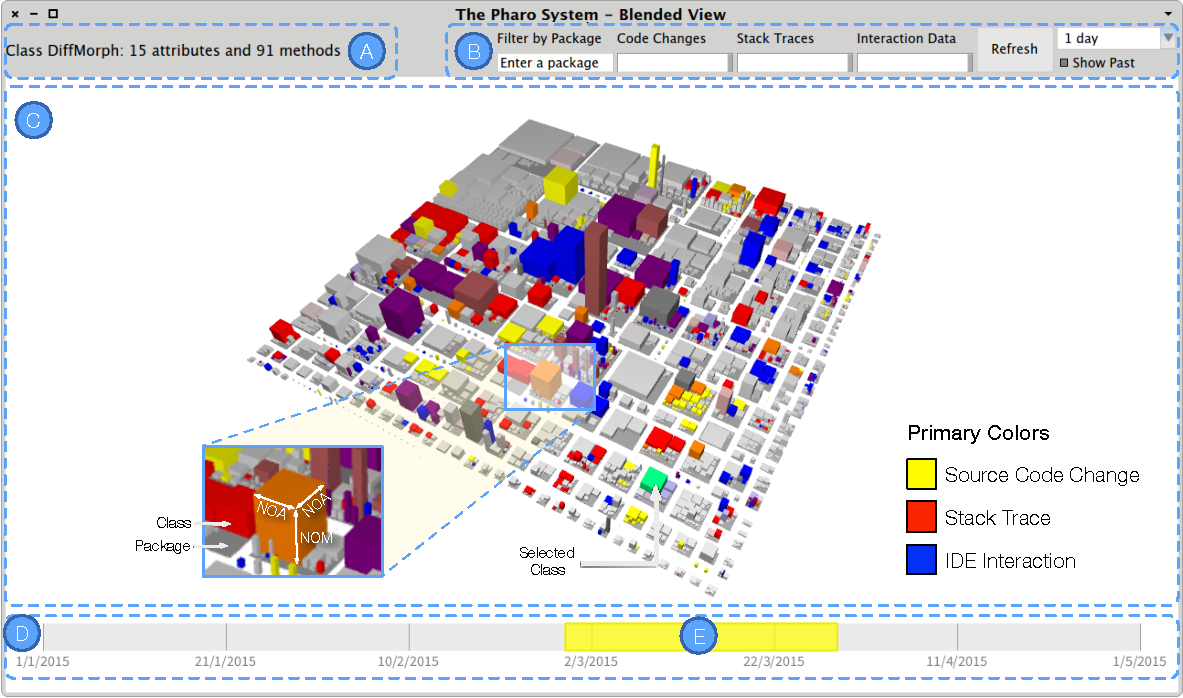
\includegraphics[width=.95\linewidth]{blend/visualization-principles}
\caption{The Blended City -- Visualization Principles and Proportions}
\label{fig:visualization-principles}
\end{figure*}

\secref{sec:blend-ingredients} introduced the three ``ingredients'' of the visualization: source code changes, stack traces, and IDE interaction data.
Until now these diverse data sources are processed and visualized in isolation, leading to an incomplete view of the system.
Our goal is to visualize all these ingredient to enable a quick and comprehensive assessment of what happened to a software system in a given time frame.
To do so, we propose the \emph{``Blended City''}, a visualization that uses the \emph{City Metaphor} to depict all the ingredients of a software system.
Wettel and Lanza initially used this metaphor in \texttt{CodeCity}, a tool that depicts software systems as cities~\cite{Wett2007}.
In addition to the structural source code information presented by \texttt{CodeCity}, our Blended City uses a mixture of colors to depict different aspects of the software system itself.
\figref{fig:visualization-principles} shows an example of our visualization.

%%%%%%%%%%%%%%%%%%%%%%%%%%%%%%%%%%%%%%%%%%%%%%%%%%%%%
\subsection{In Practice}

\figref{fig:visualization-principles} shows the tool that we implemented to visualize the Blended City.
It is composed of four main parts: A status bar to display additional information on the selected entity (Fig.~\ref{fig:visualization-principles}.A), a toolbar to customize the visualization (Fig.~\ref{fig:visualization-principles}.B), the view canvas (Fig.~\ref{fig:visualization-principles}.C), and a timeline slider (Fig.~\ref{fig:visualization-principles}.D).
With the timeline slider the user chooses the visualized data timespan.
The width (\ie granularity) of this slider can be adapted using the dropdown menu on the right part of the toolbar.
In the example of \figref{fig:visualization-principles} the user selected one month of data, starting from March 1st.
 The toolbar (Fig.~\ref{fig:visualization-principles}.B) also features a text-input and a set of sliders.
The former enables simple queries to highlight particular packages in the system while the latter let the user choose the visual weight of each of the three ingredients of our visualization.
These weights affect the intensity of the color associated to each of the ingredients.
In the example of \figref{fig:visualization-principles}, all the sliders are at 100\%, thus all the ingredients have the same importance.
\figref{fig:stack-and-half-interaction}, instead, shows the data presented in \figref{fig:visualization-principles} giving high importance to stack traces (100\%), little importance on interaction data (50\%), and no importance to source code changes.

\begin{figure}[ht]
\centering
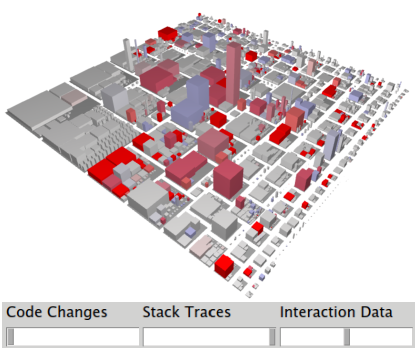
\includegraphics[width=0.8\linewidth]{blend/stack-and-half-interaction}
\caption{The Same View Depicted in \figref{fig:visualization-principles}.C with the Following Weights: 0\% Source Code Changes, 100\% Stack Traces, and 50\% Interaction Data}
\label{fig:stack-and-half-interaction}
\end{figure}

In addition to changing the weights of the three components and the granularity of the visualized timespan, the view also features standard interactions such as panning and rotation in the 3D space.
Moreover, the user can click on an entity and get additional information on the status bar.
In \figref{fig:visualization-principles} the user selected the class \texttt{DiffMorph} and the tool shows that this class has 15 attributes and 91 methods (see \figref{fig:visualization-principles}.A).
Selected entities are colored with a bright green.


%%%%%%%%%%%%%%%%%%%%%%%%%%%%%%%%%%%%%%%%%%%%%%%%%%%%%
\subsection{The City Metaphor: Layout and Metrics}

In the city metaphor every  district of the city is a package and the buildings, contained inside the districts, represent the classes~\cite{Wett2007}.
The view uses a rectangle-packing algorithm to create the layout and it is \emph{polymetric}, \ie each dimension of the visual entity is proportional to a particular metric of the program entity being represented~\cite{Lanz2004}.
Since the visualization is 3D, classes are cuboids and have 3 dimensions that correspond to three metrics.
Our visualization, similar to the original \texttt{CodeCity}, uses the same metric for both width and depth and a different measure for the height.
In particular, we use number of attributes (\ie NOA) for both width and depth of a class and number of methods (\ie NOM) for the height of the cuboid representing a class.
The magnification in \figref{fig:visualization-principles} exemplifies these mappings.

%%%%%%%%%%%%%%%%%%%%%%%%%%%%%%%%%%%%%%%%%%%%%%%%%%%%%
\subsection{Color Harmonies and Blends}

Our Blended City presents different types of data, from structural properties of source code to stack traces and interaction data.
Structural source code relationships (\ie nesting of the package and software metrics) are the foundations for the layout while colors present the remaining information.

We use a triadic color scheme made of primary colors to present this information: Yellow for source code changes, red for stack traces, and blue for interaction data.
\figref{fig:color-wheel} shows a the color wheel with an emphasis on the triadic color scheme, where colors are evenly spaced around the color wheel.

\begin{figure}[ht]
\centering
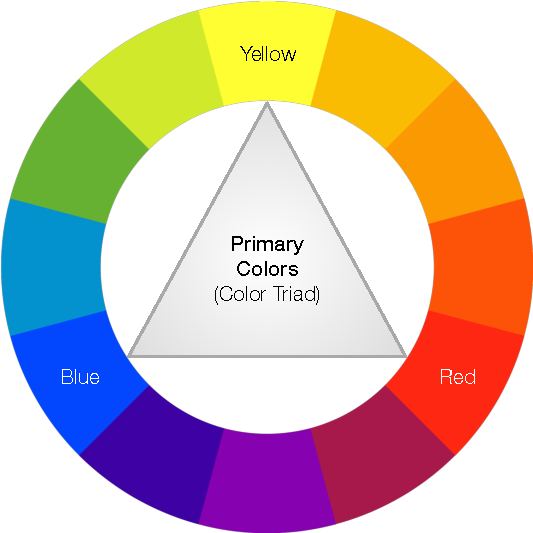
\includegraphics[width=0.4\linewidth]{blend/color-wheel}
\caption{Color Wheel and Triadic Color Scheme}
\label{fig:color-wheel}
\end{figure}

This offers strong visual contrast while retaining balance, and color richness.
Using colors equally spaced around the color wheel facilitate the addition of extra sources of information, \ie when we need to display \texttt{n} sources of information, we can create a new color harmony composed of \texttt{n} colors evenly spaced around the color wheel.


\subsubsection{Color Blends}

The three primary colors can only depict entities which are affected by a single of the three information sources.
However, in a given timespan a class might be affected by both IDE interactions and stack traces, for example when a developer is adding new functionalities to a class and testing them.
To depict this information, we use linear color blends between the different sources of information.
A class with both IDE interactions and stack traces is depicted in purple, the linear blend between the color of IDE interactions (\ie blue) and stack traces (\ie red).
\figref{fig:color-blends} shows examples of the different linear color blends on the triadic color scheme adopted by our visualization.
In this work we only considered the linear blending of colors.
It is part of our future work the investigation of different techniques to combine the colors, \ie color-weaving.

\begin{figure}[ht]
\centering
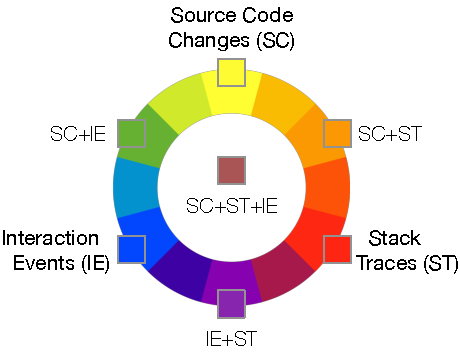
\includegraphics[width=.55\linewidth]{blend/color-blends}
\caption{Linear Color Blend on Triadic Color Scheme}
\label{fig:color-blends}
\end{figure}


\subsubsection{Aging Mechanism}

When the user selects a timespan to visualize, the tool pre-loads and displays also the data happening in the immediately preceding interval (of the same length).
This enables the user to draw conclusions from the visualization having also in mind what happened immediately before.
To show this data, the tool uses an \emph{aging mechanism} that linearly reduces the color saturation as the age of the datapoint grows, \ie the older the more intense fading towards the default color of nodes (\ie gray).
\figref{fig:color-aging-timeline} shows how colors fade with such mechanism in a timeline.

\begin{figure}[!ht]
\centering
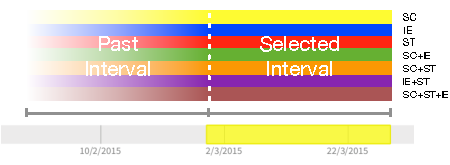
\includegraphics[width=0.9\linewidth]{blend/color-aging-timeline}
\caption{Aging Process: Example in the Timeline}
\label{fig:color-aging-timeline}
\end{figure}

%\begin{figure}[ht]
%\centering
%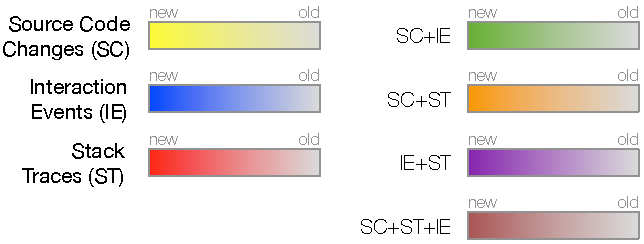
\includegraphics[width=\linewidth]{blend/color-aging}
%\caption{Aging Process: Plain and Blended Colors Fades Towards Gray}
%\label{fig:color-aging}
%\end{figure}

In the ``present'' interval (\ie the one selected by the user), colors are at their default saturation.
In the ``past''  interval, instead, the color saturation fades.
At the end of this interval, the nodes have the default color, \ie light gray.



\begin{figure*}[ht]
\centering
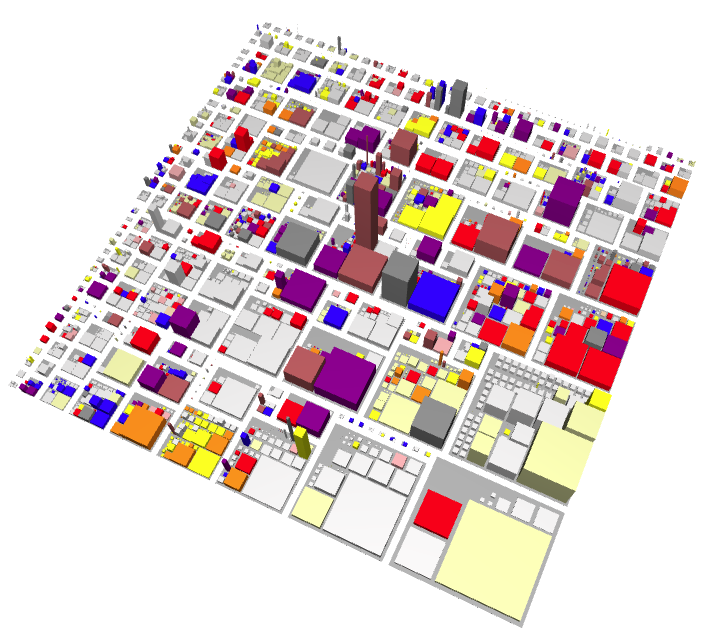
\includegraphics[width=.95\linewidth]{blend/full-view}
\caption{View of the City With All the Activities}
\label{fig:full-view}
\end{figure*}



\subsection{Under the Hood}

The tool deals with a large volume of entries coming from heterogeneous data sources.
To conveniently manage them we standardized their format, using different data pre-processors, and store them in a central place.
We use \textit{MongoDB}\seeurl{http://mongodb.org/} databases to conveniently store the data.

When the user selects a timespan to visualize (Fig.~\ref{fig:archi}.1), the tool loads the data through optimized \textit{MongoDB} queries  (Fig.~\ref{fig:archi}.2) and builds the blended model of the data  (Fig.~\ref{fig:archi}.3).
Later it computes the city layout, applies the blended color scheme, and presents the view to the user (Fig.~\ref{fig:archi}.4).
The user can then use the toolbar to refine the visualization (Fig.~\ref{fig:archi}.5).

\begin{figure}[!ht]
\centering
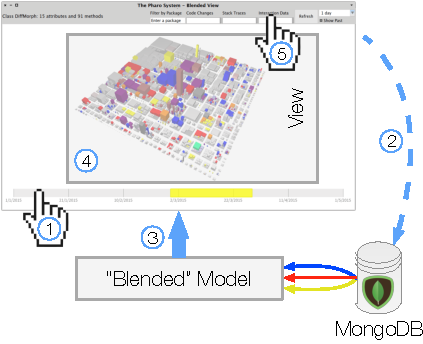
\includegraphics[width=0.75\linewidth]{blend/archi}
\caption{The Architecture of the Blended City}
\label{fig:archi}
\end{figure}



\section{Telling Evolutionary Stories}\label{sec:blend-stories}

This section presents four stories, supported by our blended view, that narrate the evolution of the \pha system.


\subsection{Those Awkward Neighbors}

By selecting the full available timespan of the data we obtain a visualization that displays all the activities that involved the \pha system over a period of five months.
This enables to obtain a comprehensive view of the system evolution and derive long-term considerations and properties.
\figref{fig:full-view} shows the overall view of the available data.
One interesting example is represented by what we call the \emph{awkward neighbors}, \ie big but silent packages that have little or no activity.

In the lower part of \figref{fig:full-view}, we can spot two big packages that contain entities that are mostly colored with grey, meaning that they had almost no activity in the whole timeframe.
Moreover, they present almost no change in the entities they are composed of, and since the color of the changes is blended, those are all antecedent to the selected start date.
This means that in the last release they have been mostly ignored.
These two districts are the packages \textit{Graphics-Files} and \textit{Compiler}, whose details are shown in \figref{fig:packages-details}.

\begin{figure}[ht]
\centering
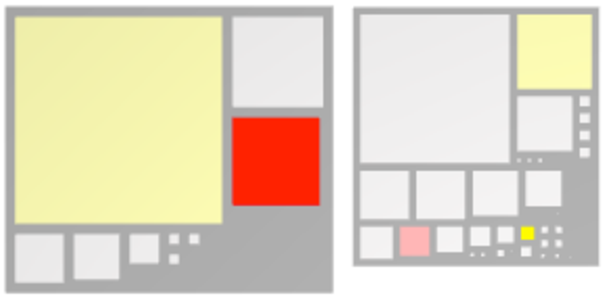
\includegraphics[width=0.6\linewidth]{blend/packages-details}
\caption{Details of the Packages \textit{Graphics-Files} and \textit{Compiler}}
\label{fig:packages-details}
\end{figure}

A further investigation of the package \textit{Graphics-Files} reveals that it contains 10 classes.
These classes are dedicated to exporting graphics and writing them in different file formats.
Since \pha stores the dates of the changes of a method, we can determine when the changes took place.
We can see that there are three main batches of changes: A small update in 2014, regarding a small refactoring of an error message, one in 2001 and one in 1997.
This is interesting, because it indicates that the package has been part of the system for a long time, it had little changes and is by now a solid foundation of the system.
Similarly, the package \textit{Compiler} contains 46 classes, and apart from some recent modification in 2013 to the structure of the compiler, many of the methods are unmodified since 2006, 2003, or 1998.

One might wonder how it is possible that some parts are older than the \pha project itself.
The reason is that \pha was born as a fork of the \textsc{Squeak} project\seeurl{http://www.squeak.org}, which in turn is a re-implementation of the original \textsc{Smalltalk-80} system, which was evolved from the \textsc{Smalltalk-72} system.
This means that some of the methods and classes in these packages might very well be 40+ years old.

%%%%%%%%%%%%%%%%%%%%%%%%%%%%%%%%%%%%%%%%%%%%%%%%%%%%%%%%%%%%
\subsection{Market Districts}

While examining some of the packages with the most activities, we found districts with many interactions from all three data sources, and we call them \emph{market districts}.
\figref{fig:market-districts} shows an example of market districts corresponding to the packages of \textit{Spec} and \textit{Morphic}.
Morphic is the core graphic library of \pha, while Spec is a framework to build user interfaces, built on top of Morphic.

\begin{figure}[ht]
\centering
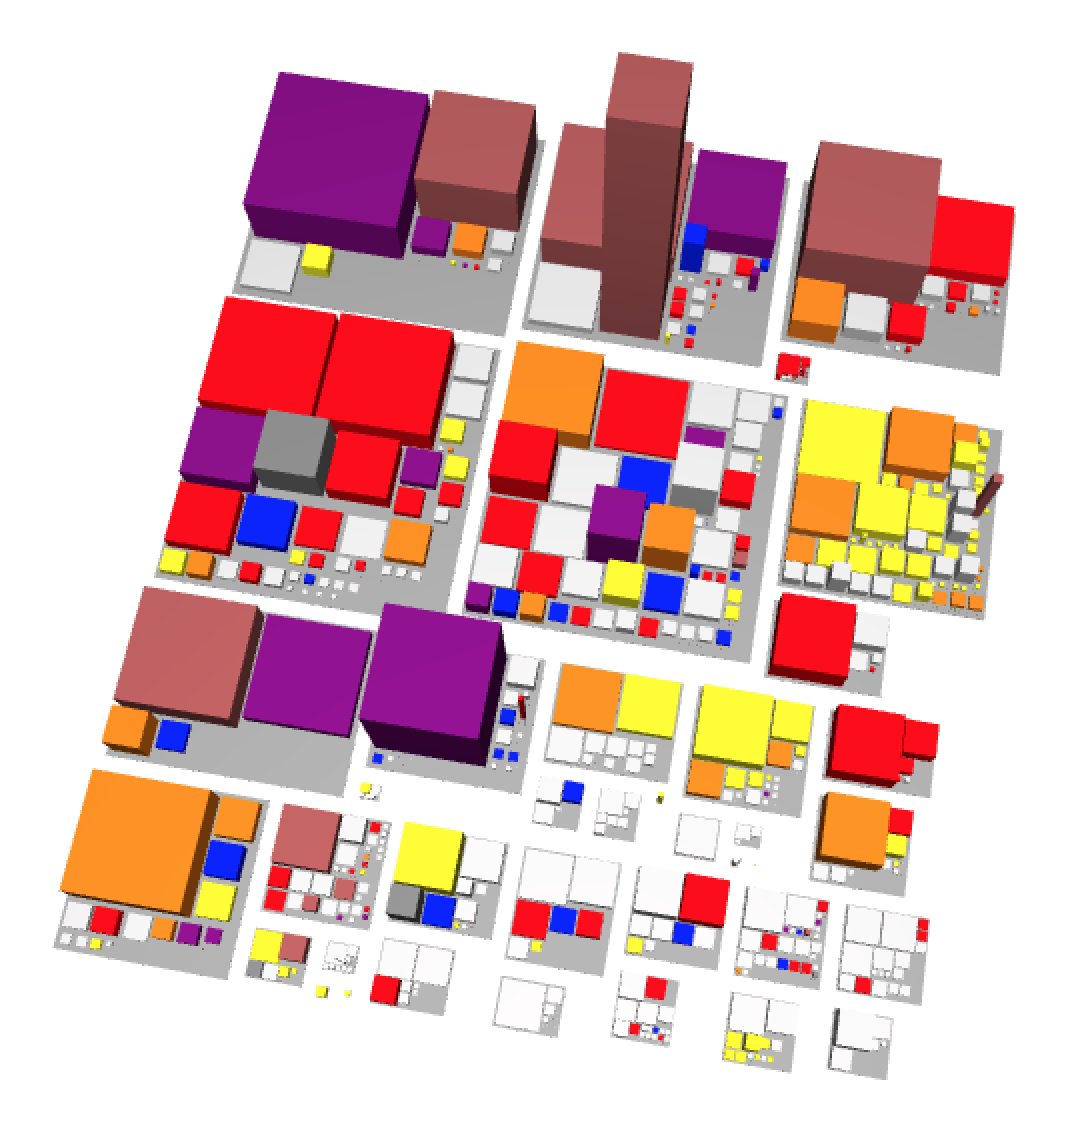
\includegraphics[width=.7\linewidth]{blend/red-district-packages}
\caption{\textit{Spec} and \textit{Morphic} Market Districts}
\label{fig:market-districts}
\end{figure}

Many classes are involved in exceptions, they were recently changed or they were subject to developer interactions.
This reveals a long known problem in the community, that is, the fact that the code of Morphic is old and have been ported through various platforms.
 The case of Spec is similar: since Spec is a framework built on top of Morphic, it shares its weakness and part of its complexities.

Differently from the awkward neighbors (shown in \figref{fig:packages-details}), the market districts for Morphic and Spec are not settled and solid: Instead, they are often causes of bugs and issues.
The view also shows that many classes that act as entry points received frequent developer interactions, meaning that they likely have an unclear public interface.

Moreover, we can see that the Morphic packages are still frequently changed, showing that the community is constantly trying to fix the codebase.
Finally, the high number of classes involved in the stack traces suggests that the code modification, together with the difficulty of understanding the API, is likely a cause of many programming errors.
In particular, there are some \emph{hotspots}, \ie packages where classes are mostly colored in red only.
These classes are involved in failures, but they are rarely modified or involved in interaction data.

These theses are confirmed by the fact that the community is trying to replace the code of Morphic with a new, polished and easy-to-use replacement called \textit{Bloc}, to address issues that we can be spot in \figref{fig:market-districts}.
However, as the complexity of the picture suggests, replacing this code is not an easy task, and has been work-in-progress for more than a year now.


%%%%%%%%%%%%%%%%%%%%%%%%%%%%%%%%%%%%%%%%%%%%%%%%%%%%%%%%%%%%

\begin{figure*}[ht]
\centering
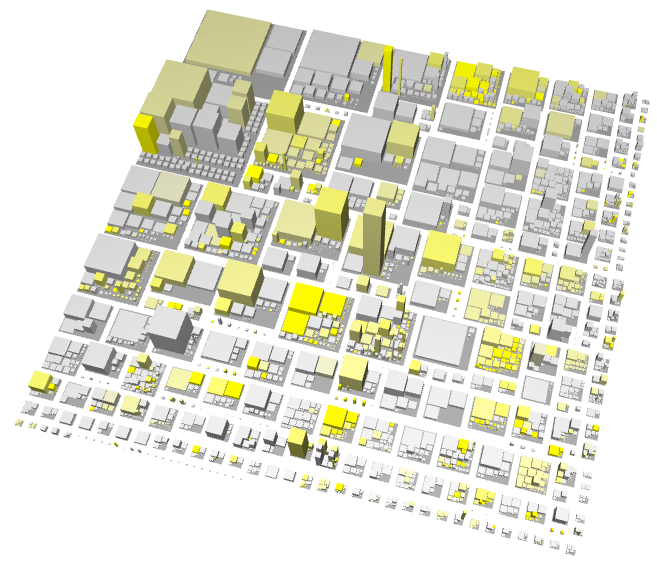
\includegraphics[width=0.75\linewidth]{blend/pharo-changes}
\caption{Changes in the Pharo System}
\label{fig:pharo-changes}
\end{figure*}

\subsection{New in Town}

During the development of Pharo 4, many classes got updated and some new components were added.
We want to analyze the progressive introduction of these changes, and how they impacted the system after the integration.
We then use the sliders in Fig.~\ref{fig:visualization-principles}.B to remove all the data sources, except for the changes.
\figref{fig:pharo-changes} shows in full yellow the entities touched by a change in the last five months, and in blended yellow the changes in the previous five months.
We can verify that there are elements that remained untouched, while some others were subject to intense development.

By moving the slider we can select a timespan to restrict the changes to a given moment of the story of the components and inspect the status of the system during time.
We can notice that from a certain point on there was the appearance of packages related to the \emph{GT-Tools}, a set of tools to improve the interaction with the objects in the system.
By restricting the timespan to the beginning of January (\ie the first appearance of activities), to determine the moment of integration.

\begin{figure}[h]
\centering
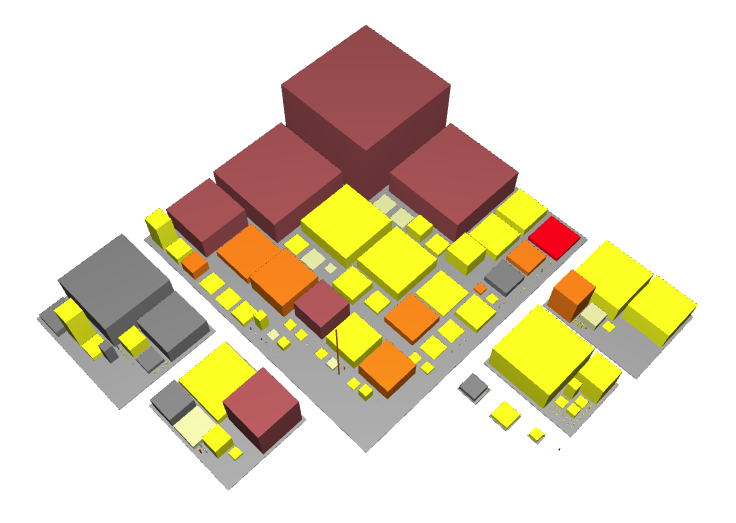
\includegraphics[width=.8\linewidth]{blend/gt-packages}
\caption{The Changes of GT-Tools Packages}
\label{fig:gt-spotter-packages}
\end{figure}

\figref{fig:gt-spotter-packages} visualizes the blended city for the \emph{GT-Tools} packages.
Some classes are involved in all three data sources, \ie they are colored in dark brown.
This can be explained by the fact that the first phases of integration usually require adaptation, refinement, and debugging, thus generating (other than changes) frequent exceptions and developer interactions.

The other interesting observation that we can derive from the visualization is that the  classes involved in user activities are also the biggest.
This can be explained by considering that those classes act as main entry points to the package, a starting point for developers who want to use or inspect the code.

%%%%%%%%%%%%%%%%%%%%%%%%%%%%%%%%%%%%%%%%%%%%%%%%%%%%%%%%%%%%

\begin{figure*}[ht]
\centering
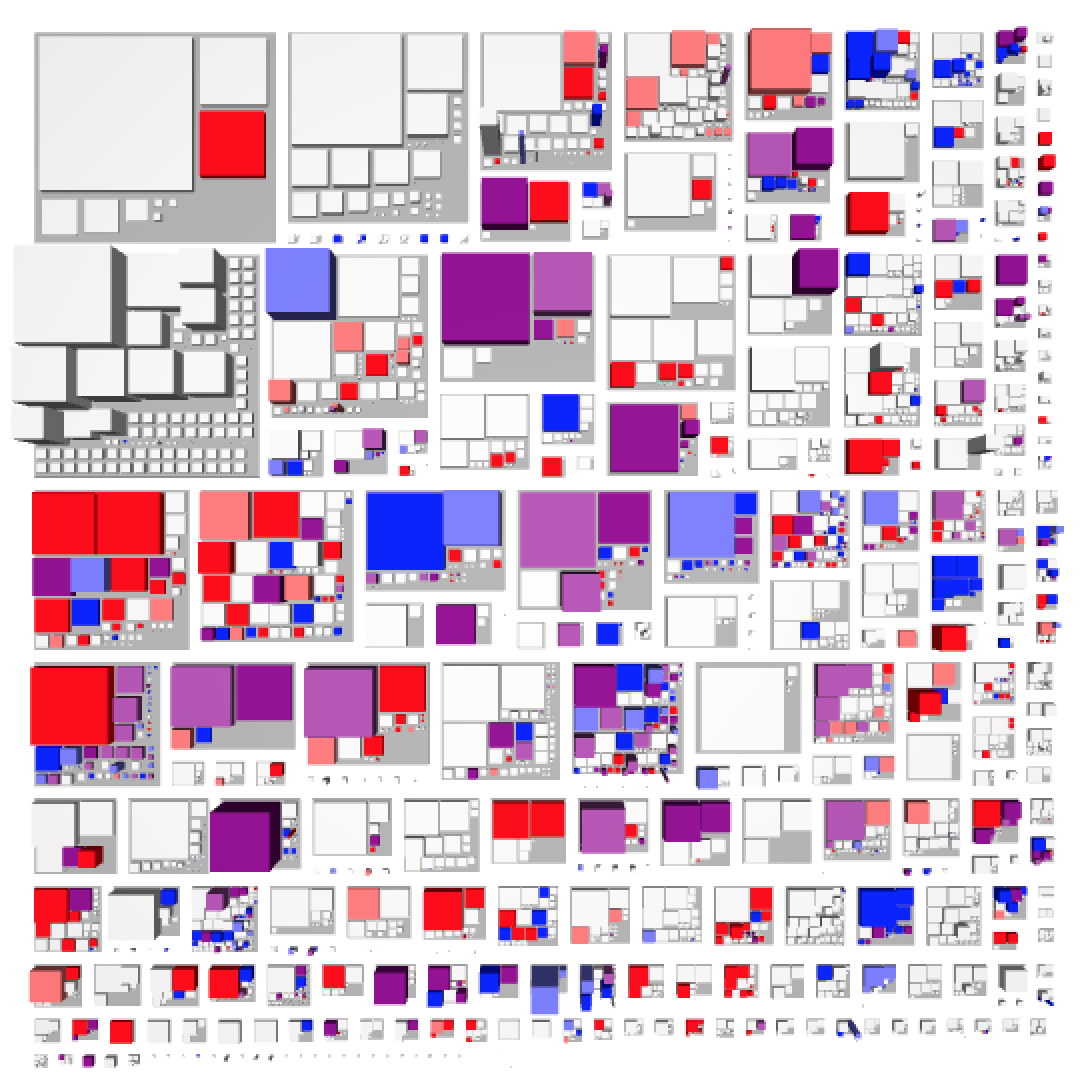
\includegraphics[width=0.9\linewidth]{blend/traces-and-interactions}
\caption{A View of the System Highlighting Stack Traces and Developer Interactions Only}
\label{fig:traces-and-interactions}
\end{figure*}

\subsection{The Purple Buildings}

A benefit of our blended city approach is that a data source can be removed to spot behaviors that are independent from it.
\figref{fig:traces-and-interactions} shows the blended city for \pha with only stack traces and developer interactions.
While the stories we presented so far try to consider the code entities at a package level,  the blended city without changes reveals the interesting role of some classes.

 Scattered across the system, there are some big and medium classes colored of purple without apparent correlation with the color of its neighbors.
By inspecting their names, we find examples like \textit{DateAndTime}, \textit{Float}, \textit{Job}, \textit{SmalltalkImage}, \textit{Socket}, \textit{SocketStream},  \textit{SystemWindow}, \textit{TestRunner}, and many others related to rendering of graphics, that we covered in the previous stories.
These classes are not problematic \emph{per se}, but represent an interesting area of the system that we could define as \emph{Advanced APIs}.
These classes appear in many stack traces and in many development interactions, an information that suggests that they occour near the source of the exceptions, when these exceptions are not directly generated from them.
This context could signify that the user is trying to understand a class that has a name suggesting a behavior, but that she needs some further understanding to learn how to use the objects of the class by trying the various methods.

The use of this information could be used by the maintainer of the system to prioritize the areas of that could need more public documentation, to ease the learning process of those entities and their API.

Note that the same information, blended with the addition of code changes and applied to classes that are not part of the core system, could signify that a developer is applying a \textit{Test Driven Development} approach, by implementing incomplete methods and completing them whenever the system tries to execute a method that is not yet implemented.



\section{Summary}\label{sec:blend-summary}

Software visualization and analysis usually focus on giving a detailed representation of a single aspect of the examined entities.
We presented an approach where we visualize data from three different data sources and contexts, blending them to produce multi-dimensional information about a system, its code and how developers interact with it.
We considered a combination of system changes during the development phase of a system, the interaction data generated by users and the stack traces of the exceptions triggered during the daily usage of the platform.

We presented a tool that visualizes our blended information on a city view of \pha, a dynamic, flexible and active programming ecosystem.
We showed how our tool allows to select different timespans and weigh the diverse components, to enable a fine grained inspection of each entity during its recent evolution.

We think that our approach has a real potential to be successfully applied in a development context to allow for multi-dimensional incremental and interactive analysis of a system, supporting a deeper understanding of the code entities by highlighting the synergies among its recorded activities, and the relations and interesting behaviors otherwise hidden or harder to detect.

We illustrated four stories where we extract and analyze some real-world issues by looking at the blending of the data and identifying some existing problems, or finding suggestions for problems that could be addressed by the maintainers of the platform to improve the system.

We believe that the knowledge highlighted by our approach can help in presenting and tackling existing problems and provide a deeper understanding of a system.

\subsection{Next Steps}

Developing out approach we became aware of many details that are hard to grasp in terms of how the users interact with the code entities.
We believe that an important next step for this analysis would be to improve the system by providing updated information on fresh data mined in real-time.

Our visualization considers activity data, but maps this information on the static entities of the system.
However, in Object Oriented Programming, the main focus lays on how these entities communicate among them, rather that how these objects are structured internally.
We think that this approach could be further improved by also considering the interactions caused by the messages sent as a result of the interactions.
%We want to deepen this perspective, and produce more refined views that could represent the true dynamic nature of a software and present a system as a network of messages correlated with the user interactions.

Finally, from the user stories we saw how to retrieve information about the evolution of the system by looking at the way users interact with it.
We think that a similar approach of combining data can be effectively put into use when analyzing old code, to understand and maintain legacy systems and support software archaeology.
